\chapter{Circuits \& Current}

\textit{Where there is power, there is resistance.}\\
\noindent\textbf{-   Michel Foucault}

\vspace{1cm}

\begin{marginfigure}%
  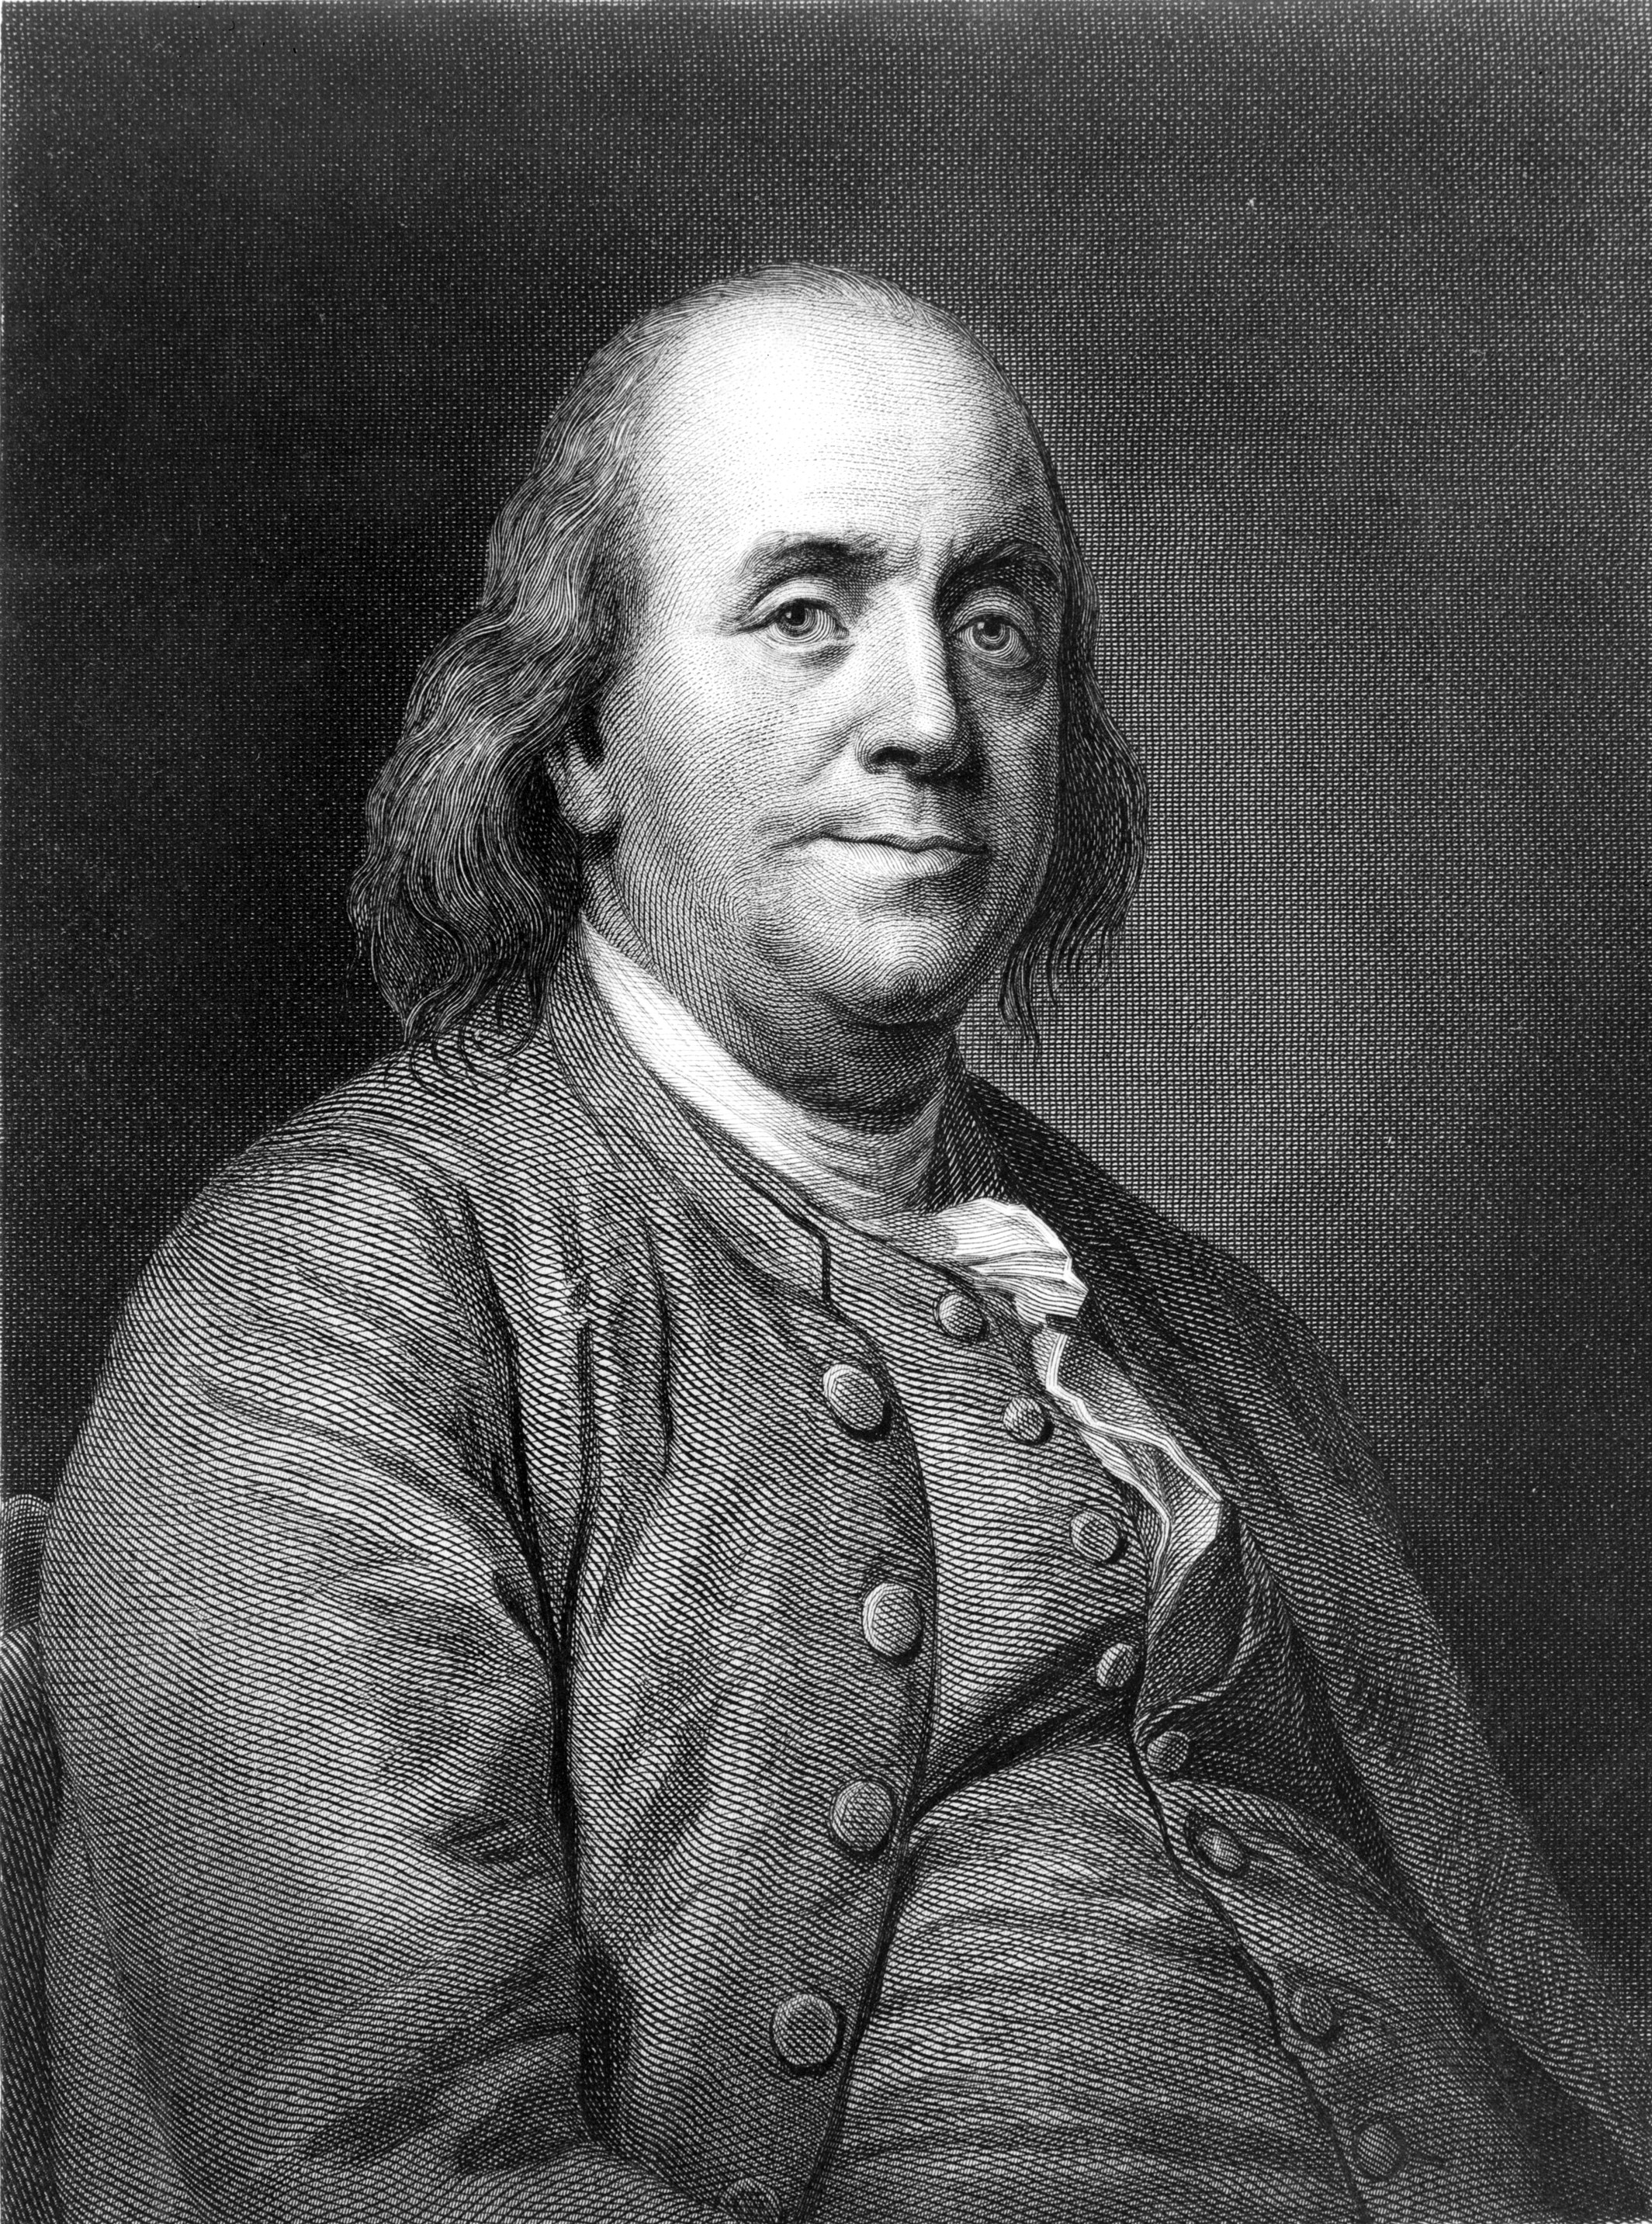
\includegraphics[width=\linewidth]{ben.jpg}
  \caption{Benjamin Franklin $\heartsuit$'s electricity}
  \label{fig:marginfig}
\end{marginfigure}

\section{Capacitance}
A capacitor holds a charge $+Q$ and $-Q$ on two plates at a given separation.   There is a voltage difference between the two plates $V$.
Capacitance is the ability of a body to store an electrical charge. A material with a large capacitance holds more electric charge at a given voltage, than one with low capacitance.  It is defined as the charge stored per volt.
$$C\equiv\frac{Q}{V}$$
The unit of capacitance is the farad.
$$1\ \text{Farad}=\frac{\text{Coulomb}}{\text{Volt}}$$
Consider the capacitor holding charges $+Q$ and $-Q$ on two plates.  Each has an area $A$ and they are separated by a distance $d$.  The constant electric field $E$ and and voltage difference $V$ are given as follows. 
$$E=\frac{\sigma}{\epsilon_0}=\frac{Q}{A\epsilon_0} \hspace{2cm} V=Ed$$
In this context the capacitance may be written in terms of the plate area and the separation distance.  
$$C=\frac{\epsilon_0A}{d}$$
In other words, the capacitance is strictly a feature of the structure of the capacitor and not a function of the particular voltage it is held at or how much charge is on it for the given conditions.

\newpage
\begin{marginfigure}%
  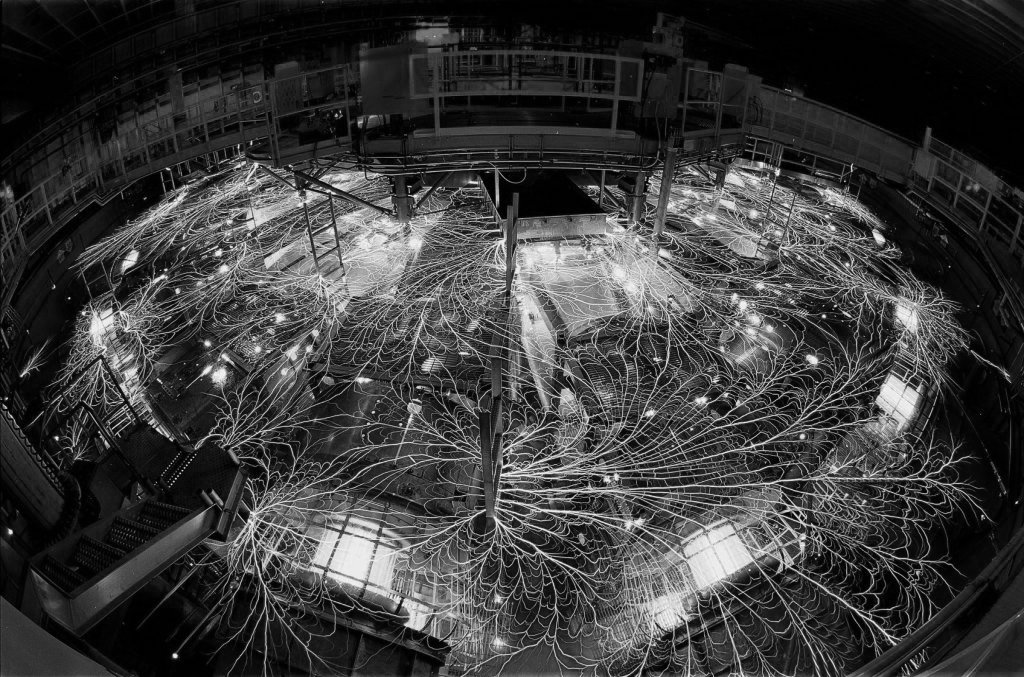
\includegraphics[width=\linewidth]{z-machine.jpg}
  \caption{The Z machine}
  \label{fig:marginfig}
\end{marginfigure}

\marginnote[30pt]{For a few billionths of a second the Z machine uses 80 times the entire world's electrical power output.}
\section{Circuit Combinations}
\subsection{Parallel}
Since the electrostatic force is conservative the voltage drop between two points should be independent of path.  Therefore the voltage drop across parallel capacitors should be equal.
$$V=V_1=V_2$$
In addition collapsing parallel capacitors into a single equivalent capacitor would have the charges add.
$$Q_{eq}=Q_1+Q_2$$
Substituting for each $Q$ using $Q=CV$ yields the next equation.
$$ C_{eq} V=C_1 V_1+C_2 V_2$$
Cancelling each of the equivalent voltages gives the following capacitance addition rule for parallel capacitors.
$$C_{eq}=C_1+C_2$$
$$\begin{circuitikz} 
\draw
(0,0) to[battery] (2,0) -- (2,2)
      to[capacitor, l=$C_1$] (0,2) -- (0,0);
      \draw (2,2) -- (2,4) to[capacitor, l=$C_2$] (0,4) -- (0,2);
\end{circuitikz}
\hspace{1cm} \text{equivalent to} \hspace{1cm} 
\begin{circuitikz} 
\draw
(0,0) to[battery] (2,0) -- (2,2)
      to[capacitor, l=$C_{eq}$] (0,2) -- (0,0);
\end{circuitikz}$$

\subsection{Series}
When capacitors are in series the voltages add to the total voltage of the circuit path.
$$V=V_1+V_2$$
The charges $Q_1$ and $Q_2$ are equal.  This is apparent when considering the floating circuit element shared by the two capacitors but completely isolated from the rest of the circuit.  Before the voltage is applied the charge in it is zero.  Once the voltage of the battery is applied the charge segregates, $+Q$ to one side and $-Q$ to the other side, conserving the total charge of zero.  Therefore the charge on the equivalent capacitor is equal to that on each of the series capacitors.
$$Q_{eq}=Q_1=Q_2$$
Starting with the voltage addition equation and substituting $V=\frac{Q}{C}$ for each component yields the following.
$$\frac{Q_{eq}}{C_{eq}}=\frac{Q_1}{C_1}+\frac{Q_2}{C_2}$$
Finally, cancelling the equal charge factors gives the equivalent capacitance for series capacitors.
$$\frac{1}{C_{eq}}=\frac{1}{C_1}+\frac{1}{C_2}$$
$$\begin{circuitikz} 
\draw
(0,0) to[battery] (4,0) -- (4,2)
      to[capacitor, l=$C_1$] (2,2) to[capacitor, l=$C_2$] (0,2) -- (0,0);
\end{circuitikz}
\hspace{1cm} \text{equivalent to} \hspace{1cm} 
\begin{circuitikz} 
\draw
(0,0) to[battery] (2,0) -- (2,2)
      to[capacitor, l=$C_{eq}$] (0,2) -- (0,0);
\end{circuitikz}$$

 
 \section{Dielectrics}
 A dielectric is a non-conductive material that increases the capacitance when placed between the two plates of a capacitor.
 $$C=\kappa C_0$$
 In such materials the $\epsilon$ replaces $\epsilon_0$.  
 $$\epsilon>\epsilon_0$$
 

\section{Energy Storage}
In order to determine the energy stored in a charged capacitor consider the small amount of work $w$ associated with adding a small amount of charge $\Delta q$ to a capacitor.
$$w=V \Delta q= \frac{q}{C}\  \Delta q$$
As more charge is added to the capacitor the voltage in the capacitor increases so the next small bit of charge requires more work to add than the previous.
$$W=\text{Area}(V(q))$$
$$PE=\frac{Q^2}{2C}=\frac{QV}{2}=\frac{CV^2}{2}$$

 \newpage
 
\section{Current}
\marginnote[0pt]{
$$1 \ \text{Ampere}=\frac{1\ \text{Coulomb}}{1\ \text{second}}$$
}
Electric current is the flow of charge.  It is the time rate of change of charge and is expressed in the unit of the ampere.
$$I \equiv \lim_{\Delta \rightarrow 0}\frac{\Delta Q}{\Delta t} \hspace{2cm} Q=\text{Area(I(t))}$$


Imagine setting up a toll both where the amount of charge flowing through the gate is counted per unit time.  This is current.
\subsection{Charge Carrier}
\marginnote[0pt]{
\begin{itemize}
\item n (carrier density)
\item q (carrier charge)
\item v (carrier velocity)
\item A (cross sectional area)
\end{itemize}
}
In electric circuits this charge is often carried by moving electrons in a wire. It can also be carried by ions in an electrolyte, or by both ions and electrons such as in a plasma.  The mobile charged body is known as the charge carrier.  The current can be determined by the number of charge carriers $N$ multiplied by the carrier charge $q$ per unit time $\Delta t$.
$$I=\frac{\Delta Q}{\Delta t}=\frac{N q}{\Delta t}$$
This can be expressed in terms of the the carrier density $n$.  This is the number of charge carriers per unit volume.
$$I=\frac{\Delta Q}{\Delta t}=\frac{n q}{\Delta t}V=nq\frac{\Delta x}{\Delta t}A=nqvA$$


\subsection{Current Density}
Current density $J$ is defined as the current passing through a cross-sectional area $A$.
$$J \equiv \frac{I}{A}=nqv$$

\section{Resistance \& Ohm's Law}
\marginnote[0pt]{
\begin{itemize}
\item $\sigma$ (conductivity)
\item $\rho$ (resistivity)
\item $l$ (length)
\item $R$ (resistance)
\end{itemize}
}
In an Ohmic material the current density is proportional to the electric field in the conductor.  The constant of proportionality $\sigma$ is known as the passivity.  
$$J=\sigma E$$
Starting fwith the above equation substitute the definition of current density and $E=\frac{V}{l}$ where $l$ is the length of the circuit element.
$$J=\frac{I}{A}=\sigma E=\sigma \frac{V}{l}$$
\marginnote[0pt]{
$$1\ \Omega=1 \ \text{Ohm}=\frac{1\ \text{Volt}}{1\ \text{Ampere}}$$
}
In circuits consisting of Ohmic materials the ratio between the voltage and the current is defined as the resistance $R$.
$$R\equiv \frac{V}{I}$$
$R$ may be expressed in terms of $\sigma$, $l$ and $A$ or the resistivity $\rho=\frac{1}{\sigma}$, the reciprocal of the passivity.
$$R=\frac{l}{\sigma A}=\rho\frac{l}{A}$$
\marginnote[-60pt]{Ohm's law is typically written as follows
$$V=IR$$}

\begin{margintable}[0pt]\index{typefaces!sizes}
  \footnotesize%
  \begin{center}
    \begin{tabular}{lc}
      \toprule
     Material & Resistivity ($\Omega\cdot \text{m}$) \\
      \midrule
     Copper     & 1.7$\times10^{-8}$  \\
    Aluminum      & 2.7$\times10^{-8}$  \\
    Tungsten (20 C)     & 5.6$\times10^{-8}$  \\
    Tungsten (1500 C)    & 5.0$\times10^{-7}$  \\
    Iron    & 9.7$\times10^{-8}$ \\
    Seawater      & 2.2$\times10^{-1}$  \\
    Blood     & 1.6  \\
    Muscle   & 1.3$\times10^{1}$  \\
    Fat      & 2.5$\times10^{1}$  \\
    Pure Water     & 2.4$\times10^{5}$  \\
    Cell Membrane     & 3.6$\times10^{7}$  \\
      \bottomrule
    \end{tabular}
  \end{center}
  \caption{A list of resistivities}
  \label{tab:font-sizes}
\end{margintable}


\section{Power}
$$P=IV$$
$$P=I^2R=\frac{V^2}{R}$$

\section{Resistors in Circuits}
\subsection{Series}
$$V=IR_1+IR_2=I(R_1+R_2)$$
$$V=IR_{eq} \hspace{2cm} R_{eq}=R_1+R_2$$

The current is the same in each resistor because any charge that flows through $R_1$ must also flow through $R_2$.

$$\begin{circuitikz} 
\draw
(0,0) to[battery] (4,0) -- (4,2)
      to[resistor, l=$R_2$] (2,2) to[resistor, l=$R_1$] (0,2) -- (0,0);
\end{circuitikz}
\hspace{1cm} \text{equivalent to} \hspace{1cm} 
\begin{circuitikz} 
\draw
(0,0) to[battery] (2,0) -- (2,2)
      to[resistor, l=$R_{eq}$] (0,2) -- (0,0);
\end{circuitikz}$$

\subsubsection{General}
$$R_{eq}=R_1+R_2+R_3 +\cdots$$

\subsection{Parallel}
The potential drop across parallel resistors is equal due to path independence of the potential function.  Additionally the total current going through each branch is conserved.
$$V=I_1R_1=I_2R_2$$
$$I=I_1+I_2$$
$$I=\frac{V}{R_1}+\frac{V}{R_2}=V\left(\frac{1}{R_1}+\frac{V}{R_1}\right)$$
$$I=\frac{V}{R_{eq}}$$
$$\frac{1}{R_{eq}}=\frac{1}{R_{1}}+\frac{1}{R_{2}}$$

$$\begin{circuitikz} 
\draw
(0,0) to[battery] (2,0) -- (2,2)
      to[resistor, l=$R_1$] (0,2) -- (0,0);
      \draw (2,2) -- (2,4) to[resistor, l=$R_2$] (0,4) -- (0,2);
\end{circuitikz}
\hspace{1cm} \text{equivalent to} \hspace{1cm} 
\begin{circuitikz} 
\draw
(0,0) to[battery] (2,0) -- (2,2)
      to[resistor, l=$R_{eq}$] (0,2) -- (0,0);
\end{circuitikz}$$
\subsubsection{General}
$$\frac{1}{R_{eq}}=\frac{1}{R_{1}}+\frac{1}{R_{2}}+\frac{1}{R_{3}}+\cdots$$

\section{Kirchoff's Rules}
\begin{itemize}
\item The sum of the currents entering a junction must be equal to the sum of the currents leaving that junction.
\item The algebraic sum of the changes in potential across all elements around any closed circuit must be zero.
\end{itemize}

\section{RC Circuits}
\marginnote[0pt]{Consider an uncharged capacitor in series with a resistor and a battery.  Initially there is no charge on it so there is no voltage drop across it.  Once the circuit is closed and the current begins to flow it begins to accumulate charge.  As it charges the rate of charging slows exponentially and approaches a maximum value asymptotically.}
$$\begin{circuitikz} 
\draw
(0,0) to[battery] (4,0) to[closing switch] (4,2)
      to[resistor, l=$R$] (2,2) to[capacitor, l=$C$] (0,2) -- (0,0);
\end{circuitikz}
$$

%$$V=V_R+V_C$$
%$$V=IR+\frac{q}{C}$$
%$$\frac{V}{R}=\frac{dq}{dt}+\frac{q}{RC}$$
%$$\int \frac{-dt}{RC}=\int \frac{dq}{q-CV}$$
\marginnote[50pt]{Consider an charged capacitor in series with a resistor and no battery.  Initially there is maximal charge on it so there maximal voltage drop across it.  Once the circuit is closed charge begins to flow of the capacitor.  As it discharges the rate slows exponentially and approaches a zero asymptotically.}
\subsection{Charging a Capacitor}
$$q(t)=CV(1-e^{-\frac{t}{RC}})=Q(1-e^{-\frac{t}{RC}})$$
$$I(t)=\frac{V}{R}e^{-\frac{t}{RC}}$$
\subsection{Discharging a Capacitor}
$$q(t)=Qe^{-\frac{t}{RC}}$$
$$I(t)=I_0e^{-\frac{t}{RC}}$$

